\section{Durchführung}
\label{sec:Durchführung}

Der verwendete Versuchsaufbau ist in Abbildung \ref{abb4} dargestellt.
\begin{figure}
    \centering
    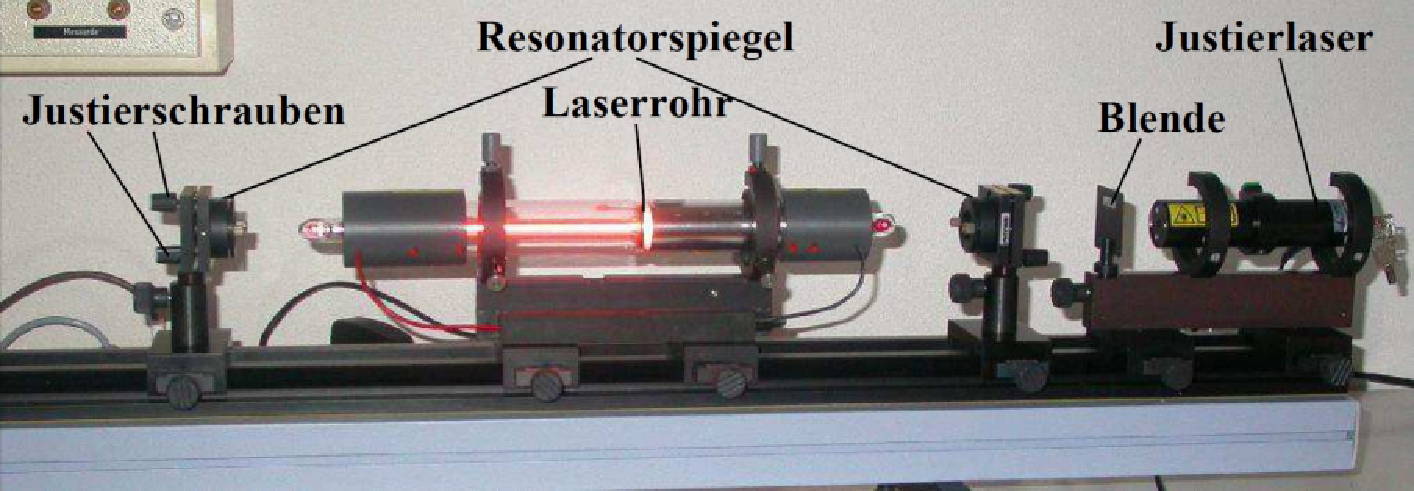
\includegraphics[width=\textwidth]{figure/Aufbau.pdf}
    \caption{Auf dieser Fotografie ist der Versuchsaufbau mit seinen 
    Hauptkomponenten abgebildet \cite{sample}.}
    \label{abb4}
\end{figure}
Der Laser befindet sich auf einer optischen Schiene zusammen mit einem grünen
Justierlaser der reduzierten Leistung $P = \SI{0,2}{\milli\watt}$.
zur Justage muss dieser grüne Laser auf eine Achse mit de optischen Bank 
gebracht werden. 
Das Laserrohr des Helium-Neon-Lasers hat eine Länge von $l = \SI{408}{\milli\meter}$
und einen Durchmesser von $d = \SI{1,1}{\milli\meter}$. Die zugehörigen 
Resonatorspiegel haben einen Durchmesser von $D = \SI{12,7}{\milli\meter}$.
Der Krümmungsradius der verwendeten konkaven Spiegel beträgt $b = \SI{140}{\centi\meter}$.
\\\\
Nach erfolgreicher Justage kann das Messprogramm gestartet werden. 
\begin{itemize}
    \item Als erstes werden die stabilitätsbedingungen für zwei konkave und für einen 
    flachen und einen konkaven Resonatorspiegelüberprüft. Dafür wird der Abstand der 
    Spiegel langsam erhöht. Für zwei konkave Spiegel wird hierbei gleichzeitig 
    das Fourierspektrum der Laserintensität mit einer Photodiode 
    für verschiedene Resonatorlängen vermessen.
    \item Danach werden die Intensitäten der $TEM_{\text{00}}$- und $TEM_{\text{10}}$-Mode
    vermessen, wobei ein Wolfram-Draht senkrecht zur Strahlachse als Modenfilter zur 
    Realisation der $TEM_{\text{10}}$-Mode in das System eingebracht wird.
    \item Als letztes wird die Polarisation des Laserlichtes bestimmt, indem ein 
    Polarisator in dem Strahl positioniert wird und die Intensität hinterm 
    Poarisator in Abhängigkeit der Polarisationsrichtung mit einer Photodiode vermessen 
    wird. 
\end{itemize}
\newpage